\section{Background}

In diesem Kapitel sollen die verwendeten Bibliotheken und der Grund für ihre Verwendung genauer beleuchtet werden. Damit Daten generiert werden konnten, wurde die Bibliothek \textit{GetOldTweets3} verwendet. Mit einer öffentlich zugänglichen Userliste für Politiker aus Amerika wurden mithife dieser Packages die Daten erhoben. Zur Weiterverarbeitung der Daten wurden \textit{NLTK} und \textit{TextBlob} genutzt. Beides sind Tools für die Verarbeitung von Sprache. Um eine Analyse über die verarbeiteten Ausgaben durch ein MapReduce laufen zu lassen, wurde schließlich Spark verwendet, um eine Zeit effiziente Verarbeitung zu gewährleisten.
	
\subsection{GetOldTweets3-Pakage}
	
\textit{GetOldTweets3} ist ein kostenloses Python 3 Package mit welchem Twitterdaten ohne API-Schlüssel abgerufen werden können. Mit \textit{GetOldTweets3} können Tweets mit einer Vielzahl von Suchparametern wie Start-/Enddatum, Benutzername(n), Textabfrage und Referenzortbereich extrahiert werden. Außerdem können Tweet-Attribute die einbezogen werden sollen berücksichtigt werden. Beispielsattribute sind Folgende: Nutzername, Tweettext, Datum, Retweets und Hashtags \citeint{userguid}. Die offizielle API von Twitter hat ein beschränktes Zeitfenster, weshalb keine Tweets älter als eine Woche abgerufen werden können. Es gibt einige Tools, die Zugang zu älteren Tweets anbieten, diese sind jedoch meistens kostenpflichtig. Das Forschungsteam hat nach einem anderen Tool gesucht um diese Aufgaben zu übernehmen, wodurch die Wahl auf das Package  \textit{GetOldTweets3} gefallen ist \citeint{python}.

Die Analyse des Codes von \textit{GetOldTweets3} und die Funktionsweise des Searchthrough Browsers von Twitter zeigt, wie das Package auch an alte Tweets kommt. Wenn auf Twitter Seiten oder User gesucht werden, startet ein Scroll-Loader. Das heißt, beim scrollen nach unten, tauchen immer mehr Tweets zu den jeweiligen Suchparametern auf. Diese Tweets bekommen sie durch Abfragen an einen JSON-Provider. \textit{GetOldTweets3} imitiert den Searchthrough Browser von Twitter um den Scroll-Loader zu starten und zieht sich dann anhand der Abfragen an einen JSON-Provider die JSON-Datei und gibt diese decodiert zurück um somit alle Tweets anhand der oben gegebenen Parameter herauszufiltern. Dies kann man in dem Github-Repository gut nachvollziehen \citeint{github}. Somit ist es möglich, sowohl aktuelle als auch sehr alte Tweets zu scrapen.
	
	
	\begin{figure}[ht]
		\centering
		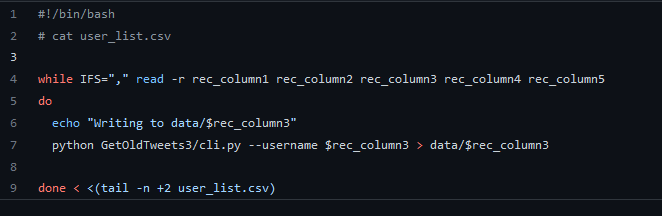
\includegraphics[width=0.9\textwidth]{images/Kapitel2/Code_Beispiel_1}
			\caption{\label{fig:CodeBeispiel}Code Beispiel für das Scrapen der Tweets}{Ist eine Python Bibliothek mit der Twitter Daten durch den Scroll-Loader des Searchthrough Browsers von Twitter als JSON-Datei abgerufen werden können.}
	\end{figure}
	
So kann durch eine paar Zeilen Code, wie man in der Abbildung \label{CodeBeispiel} erkennen kann, eine Bash-Datei erstellt werden, durch welche die Daten gesucht und abgespeichert werden. Das Scraping kann durch die Größe der JSON-Datei einige Zeit in Anspruch nehmen. Wir haben für 2 Millionen Tweets insgesamt eine Laufzeit von ca. 35 Stunden verbucht.

	\subsection{NLTK-Natural language Toolkit}
	
\textit{NLTK} ist ein Pythonpackage für die Arbeit mit menschlichen Sprachdaten. Es bietet einfach zu bedienende Schnittstellen zu über 50 Korpora und lexikalischen Ressourcen wie WordNet, zusammen mit einer Reihe von Textverarbeitungsbibliotheken für Klassifizierung, Tokenisierung, Stemming, Tagging, Parsing und semantische Schlussfolgerungen sowie Wrapper für industrielle NLP-Bibliotheken und ein aktives Diskussionsforum \citeint{nltk}.
	
	
Aus diesem Grund bietet \textit{NLTK} sehr viele Möglichkeiten zur Vorverarbeitung und Analyse, benötigt aber auch einen gewissen Zeitrahmen zur Einarbeitung in die Analysen. Aus diesem Grund hat sich das Forscherteam dafür entschieden, NLTK nur zur Vorverarbeitung zu nutzen und TextBlob für die semantische Analyse zu nutzen. Warum sich für TextBlob entschieden wurde, wird genauer in 2.1.3 besprochen. So verwenden wir den Wordkorpus von NLTK für englische Stoppworte, da diese nicht Teil der Analyse sein sollen.
	
Für eine individuelle und sehr ausführliche semantische Analyse bietet NLTK sehr viele Möglichkeiten durch die Interaktion mit verschiedenen Packages in Python, was aber den oben genannten Zeitrahmen benötigt, zum Einarbeiten. Der Vorteil von NLTK gegenüber TextBlob sind genau diese Interaktionen mit anderen Packages. Für größere Projekte, bei denen man die semantische Analyse auch individuell anpassen möchte, sollte man die NLTK Bibliothek benutzen. NLTK ermöglicht es durch verschiedene Vorverarbeitungsschritte, welche in der Bibliothek eingebaut sind, eine individuelle Pipeline und Analyse zu erstellen.
	
	\begin{figure}[ht]
		\centering
		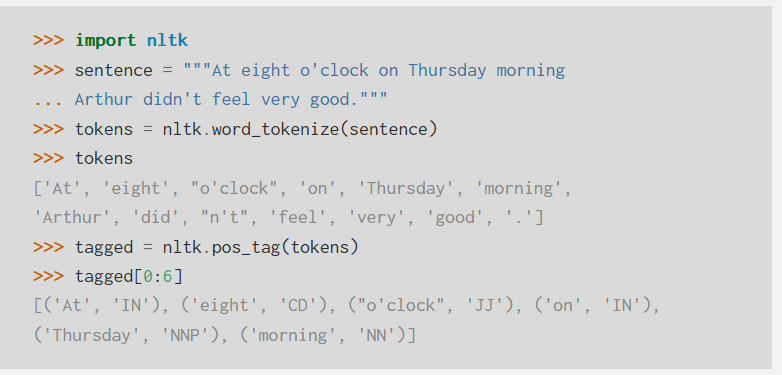
\includegraphics[width=0.9\textwidth]{images/Kapitel2/Code_Beispiel_2}
			\caption{\label{fig:CodeBeispiel}Code Beispiel für das Arbeiten mit NLTK}{Tokenisierung und Tagging von Texten mit NLTK}
	\end{figure}
	
	\subsection{TextBlob}
	
TextBlob ist eine Python Bibliothek für Python zwei und drei. Diesem Package arbeiten, ähnlich wie NLTK, mit verschiedenen Packages, welche in Python schon verfügbar sind. In TextBlob sind zwei verschiedene semantische Analysen vorhanden. Da gibt es zum einen die Patternanalyse verwendet, welche die Pattern Bibliothek in Python nutzt, und dann gibt es da noch die Naive-Bayes-Analyse \citeint{blob}. Hier stellt NLTK zum Beispiel mehr zur Verfügung, aber benötigt damit auch mehr Einarbeitungszeit. Damit bietet TextBlob eine besser Übersicht, weshalb sich das Forschungsteam aufgrund der wenigen Zeit für diese Bibliothek entschieden hat.
	
Ein weiter Grund, warum sich schlussendlich für diese Bibliothek entscheiden wurde, sind auch die zwei Outputwerte Polarität und Subjektivität welche eine gute Anwendungsmöglichkeit darstellen \citeint{userguideText}. In der Analyse haben wir die Patternanalyse von TextBlob verwendet, welche uns die Polarität in einem Intervall von [-1, 1] und die Subjektivität im Rahmen von [0, 1] zurück gibt. Ist der Wert bei der Polarität näher an der -1 als an der 1, dann zeigt es einen negative Emotion. Im umgekehrten Fall ist es eine positive Emotion.
	
Bei dem Wert der Subjektivität beschreibt ein Wert, der gegen null tendiert, einen Fakt oder Faktenwissen und eine Tendenz gegen eins entspricht einer stärkeren subjektive Meinung mit rein \citeint{semtiment} \citeint{blobkgit}. Bei der Patternanalyse geht es darum, ein Muster bei negativen und positiven Aussagen zu erkennen und dies dann auf neue Testdaten oder unbekannte Daten anzuwenden. Dabei spielt sowohl die Syntax als auch die Semantik und die Wortwahl eine bedeutende Rolle \citeint{pattern}. Mit etwas mehr Zeit hätte man auch noch die Analyse des Naive-Bayes in einem MapReduce verwenden können.

	
	\subsection{Spark}
	
Spark ist ein Big Data Framework zur Verarbeitung, Filterung und Analyse von großen Datenmengen. Diese Bibliothek vereinfacht die Anwendung eines MapReduce, indem es verschiedene Funktionsweisen und Tools dafür anbietet. So begrenzt sich der Programmcode auf die wesentlichen Funktionen eines MapReduce und verschafft dadurch eine guet Übersicht über den Code. Des Weiteren stellt Spark verschiedene Datenstrukturen zur Verfügung, um die Arbeit mit großen Datenmengen zu erleichtern. Dazu gehört zum Beispiel das Resilient Distributed Datasets (RDD). Ein weiter Vorteil, den Spark bietet, ist die hohe Verarbeitungsgeschwindigkeit der Daten. Aus diesen Gründen hat sich das Forscherteam für das Mapreduce entschieden, welches in dem Forschungsprojekt Anwendung finden soll, diese Bibliothek zu verwenden, um eine einfach und zeit effiziente Verarbeitung der Twitterdaten zu haben.
	    
	

	
